\documentclass[12pt,a4paper,oneside]{article}
\usepackage[utf8]{vietnam}
\usepackage{amsmath}
\usepackage{amsfonts}
\usepackage{amssymb}
\usepackage{graphicx}
\usepackage[left=2cm,right=2cm,top=2cm,bottom=2cm]{geometry}
\usepackage{array}
\usepackage{fancyhdr}
\pagestyle{fancy}
\renewcommand\thesection{\Roman{section}.}
\renewcommand\thesubsection{\arabic{subsection}.}
\fancyhf{}
\rhead{Week 4}
\lhead{Hoàng Quốc Bảo - 20194484}
\rfoot{Trang \thepage}

\usepackage{listings}
\usepackage{tcolorbox}
\usepackage{color} % tô màu cho code
\definecolor{dkgreen}{rgb}{0,0.6,0}
\definecolor{gray}{rgb}{0.5,0.5,0.5}
\definecolor{mauve}{rgb}{0.58,0,0.82}
\lstset{frame=tb,
  language=[x86masm]Assembler,
  aboveskip=3mm,
  belowskip=3mm,
  showstringspaces=false,
  columns=flexible,
  basicstyle={\small\ttfamily},
  backgroundcolor=\color{gray!20!white},
  numbers=none,
  breaklines=true,
  breakatwhitespace=true,
  tabsize=3
}

\begin{document}
\section*{Assignment 1}
\textbf{Mã nguồn:}
\begin{lstlisting}
#Laboratory Exercise 4, Home Assignment 1
.text
start:
li $t0,0 #No Overflow is default status
li $s1, 2019448420194484
li $s2, 20194484
addu $s3,$s1,$s2 # s3 = s1 + s2
xor $t1,$s1,$s2 #Test if $s1 and $s2 have the same sign

bltz $t1,EXIT #If not, exit
slt $t2,$s3,$s1
bltz $s1,NEGATIVE #Test if $s1 and $s2 is negative?
beq $t2,$zero,EXIT #s1 and $s2 are positive
 # if $s3 > $s1 then the result is not overflow
j OVERFLOW
NEGATIVE:
bne $t2,$zero,EXIT #s1 and $s2 are negative
 # if $s3 < $s1 then the result is not overflow
OVERFLOW:
li $t0,1 #the result is overflow
EXIT:

\end{lstlisting}
\textbf{Quan sát giá trị các thanh ghi}
\begin{itemize}
\item 4 lệnh đầu tiên khởi tạo giá trị cho các thanh ghi\quad 
\includegraphics[scale=1]{1.1}.
\item Lệnh 
\includegraphics[scale=1]{1.2} nhằm xác định xem giá trị thanh ghi \$s1, \$s2 có cùng dấu với nhau hay không. \textit{(Nếu cùng dấu thì giá trị bit đầu tiên của \$s1 và \$s2 sẽ cùng bằng 0 hoặc cùng bằng 1. Lúc đó khi xor giá trị 2 bit đầu tiên với nhau sẽ cho ra kết quả có bit đầu tiên = 1 => Giá trị thanh ghi \$t0 \linebreak sẽ < 0 và ngược lại, nếu 2 giá trị thanh ghi \$s1 và \$s2 khác dấu thì giá trị của thanh \linebreak ghi \$t0 sẽ > 0)}\\\textit{Ở đây, do 2 thanh ghi đều là số dương nên giá trị thanh ghi \$t1 sẽ có bit đầu tiên = 1.} \begin{center}
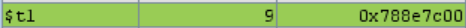
\includegraphics[scale=1]{1.4}
\end{center}
\item Lệnh 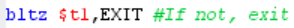
\includegraphics[scale=1]{1.3} thực hiện rẽ nhánh. Nếu 2 thanh ghi \$s1 và \$s2 khác dấu thì không thể có hiện tượng tràn số => Kết thúc chương trình.\\\textit{Ở đây, 2 thanh ghi cùng dấu nên lệnh này bỏ qua.}
\item Lệnh 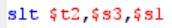
\includegraphics[scale=1]{1.5} so sánh kết quả \$s3 và \$s1. \\\textit{Ở đây, ta có giá trị \$t2 = 0 do \$s3 > \$s1}.
\begin{center}
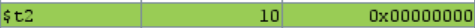
\includegraphics[scale=1]{1.6}
\end{center}
\item Lệnh 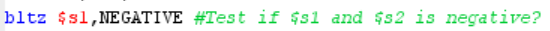
\includegraphics[scale=1]{1.7} thực hiện rẽ nhánh đến nhãn NEGATIVE nếu \$s1 và \$s2 < 0.\\\textit{Ở đây, lệnh này bị bỏ qua do \$s1 và \$s2 > 0}
\item Lệnh 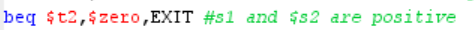
\includegraphics[scale=1]{1.8} thực hiện rẽ nhánh đến nhãn EXIT (kết thúc chương trình) nếu thanh ghi \$t2 = 0.\\\textit{Ở đây, lệnh này được thực hiện và chương trình kết thúc. Do thanh ghi \$t2 chứa kết quả so sánh giữa thanh ghi \$s3 và \$s1. Vì thanh ghi \$s3 > \$s1 nên ta kết luận không bị tràn bit. (Nếu tràn bit thì thanh ghi \$s3 sẽ bị mất bit dẫn đến \$s3 < \$s1).}
\end{itemize}



\pagebreak
\section*{Assignment 2}
\subsection*{a) Extract MSB of \$s0}
\textbf{Mã nguồn}
\begin{lstlisting}
#Laboratory Exercise 4, Home Assignment 2a
#Extract MSB of $s0
.text
li $s0, 0x20194484 #load test value for these function
andi $t0, $s0, 0xff000000 #Extract the MSB of $s0
\end{lstlisting}
\textbf{Giải thích:} Phép and giữ nguyên một số bit, các bit còn lại = 0. Vậy muốn giữ lại 8 bit bên trái (MSB) thì ta chỉ cần and với mặt nạ có giá trị các bit = 1 ở 8 bit bên trái là được. \\\\
\textit{Giá trị thanh ghi \$s0: \quad 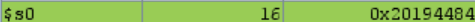
\includegraphics[scale=1]{2.0}}\\
\textit{Kết quả thu được: \quad \quad 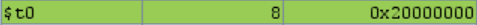
\includegraphics[scale=1]{2.1}}


\subsection*{b) Clear LSB of \$s0}
\textbf{Mã nguồn}
\begin{lstlisting}
#Laboratory Exercise 4, Home Assignment 2b
#Clear LSB of $s0
.text
li $s0, 0x20194484 #load test value for these function
andi $s0, $s0, 0xffffff00 #Clear LSB of $s0
\end{lstlisting}
\textbf{Giải thích:} Muốn xoá 8 bit bên phải (LSB) và giữ nguyên các bit còn lại thì ta chỉ cần and với mặt nạ có giá trị = 0 ở 8 bit bên phải và các bit còn lại = 1 là được.  \\\\
\textit{Giá trị thanh ghi \$s0: \quad 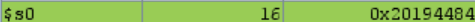
\includegraphics[scale=1]{2.0}}\\
\textit{Kết quả thu được: \quad \quad 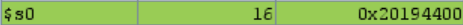
\includegraphics[scale=1]{2.2}}

\subsection*{c) Set LSB of \$s0 (bits 7 to 0 are set to 1)}
\textbf{Mã nguồn}
\begin{lstlisting}
#Laboratory Exercise 4, Home Assignment 2c
# Set LSB of $s0 (bits 7 to 0 are set to 1)
.text
li $s0, 0x20194484 #load test value for these function
ori $s0, $s0, 0x000000ff # Set LSB of $s0 (bits 7 to 0 are set to 1)
\end{lstlisting}
\textbf{Giải thích:} Phép or đặt một số bit = 1, còn lại giữ nguyên. Vậy nếu muốn đặt 8 bit bên phải (LSB) = 1 thì ta chỉ cần or với mặt nạ có 8 bit bên phải = 1, các bit còn lại = 0 là được.  \\\\
\textit{Giá trị thanh ghi \$s0: \quad 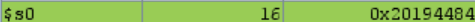
\includegraphics[scale=1]{2.0}}\\
\textit{Kết quả thu được: \quad \quad 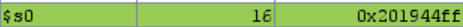
\includegraphics[scale=1]{2.3}}
\pagebreak
\subsection*{d) Clear \$s0 (\$s0=0, must use logical instructions)}
\textbf{Mã nguồn}
\begin{lstlisting}
#Laboratory Exercise 4, Home Assignment 2d
# Clear $s0 (s0=0, must use logical instructions)
.text
li $s0, 0x20194484 #load test value for these function
andi $s0, $s0, 0x00000000 # Clear $s0
\end{lstlisting}
\textbf{Giải thích: } Muốn đặt tất cả bit của \$s0 về 0 thì chỉ cần and với mặt nạ chứa toàn bit 0 là được. \\\\
\textit{Giá trị thanh ghi \$s0: \quad 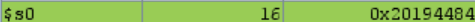
\includegraphics[scale=1]{2.0}}\\
\textit{Kết quả thu được: \quad \quad 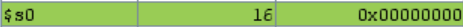
\includegraphics[scale=1]{2.4}}



\pagebreak
\section*{Assignment 3}
	\subsection*{a) abs \$s0, \$s1}
	\begin{center}
	\begin{lstlisting}
#Laboratory Exercise 4, Home Assignment 4a 
#abs $s0,s1 - convert to real-instructions of MIPS	
# 20194484
.text
addiu $s1, $zero, -3 # load test value word
addiu $s3, $zero, 0xffffffff # $s3 store 0xffffffff value
bltz $s1, else # Branch if $s1 < 0
add $s0, $s1, $zero # $s0 = $s1
j done
else:
addi $s0, $s1, -1   # $s0 = $s1 - 1
xor $s0, $s0, $s3   # Bit invert $s0
done:
	\end{lstlisting}
	\end{center}
	\textbf{Giải thích:\\}
	Thanh ghi \$s1 chứa giá trị cần lấy giá trị tuyệt đối. Thanh ghi \$s3 chứa 32 bit 1 (để phục vụ cho việc đảo bit).\\
	Ta thực hiện so sánh giá trị thanh ghi \$s1 với 0. Nếu \$s1 >= 0 thì gán \$s0 = \$s1 và kết thúc chương trình.\\ Nếu \$s1 < 0 thì ta trừ 1 bit cho \$s1 và xor với \$s3 để thực hiện đảo bit. Kết quả thu được lưu vào \$0.
	
	\subsection*{b) move \$s0, \$s1}
	\begin{center}
	\begin{lstlisting}
#Laboratory Exercise 4, Home Assignment 4b
#move $s0,s1 - convert to real-instructions of MIPS
# 20194484
addi $s1, $s1, -4484	# Load test value of $s1
add $s0, $zero, $s1		# $s0 = $s1

	\end{lstlisting}
	\end{center}
	\textbf{Giải thích:\\}
	Lệnh move thực hiện sao chép nội dung từ thanh ghi \$s1 sang thanh ghi \$s0. Ta sử dụng cách thay thế bằng biểu thức \$s0 = \$s1 + 0.
	
	\subsection*{c) not \$s0,s1}
	\begin{center}
	\begin{lstlisting}
#Laboratory Exercise 4, Home Assignment 4c
#not $s0,s1 - convert to real-instructions of MIPS
# 20194484
.text
addiu $s1, $zero, 4484 # load test value word
addiu $s3, $zero, 0xffffffff # $s3 store 0xffffffff value
xor $s0, $s1, $s3	# $s0 = invert bit of $s1

	\end{lstlisting}
	\end{center}
	\textbf{Giải thích:\\}
	Lưu giá trị \$s3 chứa 32 bit 1. Vậy khi xor \$s1 với \$s3, ta sẽ thu được giá trị là đảo của \$s1.
	
	\subsection*{d) ble \$s1,\$s2,L}
	\begin{center}
	\begin{lstlisting}
#Laboratory Exercise 4, Home Assignment 4d
# ble $s1,s2,L - convert to real-instructions of MIPS
# 20194484
addi $s1, $zero, 2019
addi $s2, $zero, 4484
slt $s0, $s1, $s2  # $s0 = 1 if $s1 < $s2
bne $s0, $zero, L  # if $s0 = 1 then branch to L 
addi $t1, $zero, 1 # if $s1 > $s2 then $t1 = 1
j done
L:
addi $t1, $zero, 2 # if $s1 < $s2 then $t1 = 2
done:

	\end{lstlisting}
	\end{center}
	\textbf{Giải thích:\\}
	Ta chuyển lệnh ble thành 2 lệnh slt và bne.\\
	Lệnh ble sẽ thực hiện nhảy đến nhãn L nếu \$s1 < \$s2.\\
	Lệnh slt sẽ gán \$s0 = 1 nếu \$s1 < \$s2 và lệnh bne sẽ nhảy đến nhãn L nếu \$s0 = 1. (Thanh ghi \$t1 để check kết quả). Nếu \$s1 > \$s2 thì \$t1 = 1. Nếu \$s1 < \$s2 thì \$t1 = 2.
	

\pagebreak
\section*{Assignment 5}
\textbf{Mã nguồn}
\begin{lstlisting}
#Laboratory Exercise 4, Assignment 5
# Write a program that implement multiply by a small power of 2. (2, 4, 8, 16, ...)
.text
li $t0 4 	# $t0 is factor
li $s0 4484	# $s0 is factor
repeat:
srl $t0, $t0, 1
beq $t0, $zero, exit
sll $s0, $s0, 1
j repeat
exit:
\end{lstlisting}
\textit{Kết quả thực hiện: \quad 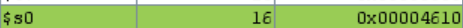
\includegraphics[scale=1]{5}}\\\\
\textbf{Giải thích: } Sau mỗi lần lặp thì \$t0 sẽ bị giảm đi một nửa (dịch phải 1 bit), \$s0 sẽ tăng lên gấp đối (dịch trái 1 bit). Cứ lặp như vậy đến khi \$t0 = 0 thì giá trị \$s0 sẽ là kết quả cần tìm.

\end{document}